\notechapter{N-20260304}{Point-Set Language in \texorpdfstring{$\mathbb R^n$}{Rn}: Neighborhoods, Boundaries, and Compactness}

\section{Why point-set language appears}

In one-variable calculus, the domain is often an interval, so the topology is mostly hidden.  In several variables, a domain may have holes, corners, isolated points, missing boundary pieces, or several connected components.  Pictures help, but pictures can lie.  The reliable language is the language of balls, neighborhoods, boundary points, and sequences.

Throughout this note, points are in \(\mathbb R^n\), and distance means Euclidean distance:
\[
  \rho(P,Q)=\norm{P-Q}_2
  =\sqrt{\sum_{i=1}^n(p_i-q_i)^2}.
\]

\section{Balls and neighborhoods}

\begin{definition}
For \(P_0\in\mathbb R^n\) and \(\delta>0\), the open ball of radius \(\delta\) around \(P_0\) is
\[
  B_\delta(P_0)=\{P\in\mathbb R^n:\rho(P,P_0)<\delta\}.
\]
A set \(U\) is a \vocab{neighborhood} of \(P_0\) if it contains some open ball \(B_\delta(P_0)\).
\end{definition}

A neighborhood is the formal version of "all points sufficiently close to \(P_0\)."  This phrase is the engine behind limits, continuity, differentiability, and local extrema.

\begin{example}
In \(\mathbb R^2\), the disk
\[
  D=\{(x,y):x^2+y^2<1\}
\]
is a neighborhood of \((0,0)\), because it contains \(B_{1/2}(0,0)\).  The punctured disk
\[
  D\setminus\{(0,0)\}
\]
is not a neighborhood of \((0,0)\), although every small ball around the origin meets it.
\end{example}

\section{Interior, exterior, and boundary}

\begin{definition}
Let \(E\subseteq\mathbb R^n\).  A point \(P\) is
\begin{enumerate}[(i)]
  \item an \vocab{interior point} of \(E\) if some ball around \(P\) is contained in \(E\);
  \item an \vocab{exterior point} of \(E\) if some ball around \(P\) is disjoint from \(E\);
  \item a \vocab{boundary point} of \(E\) if every ball around \(P\) meets both \(E\) and \(\mathbb R^n\setminus E\).
\end{enumerate}
The set of all boundary points is denoted \(\partial E\).
\end{definition}

These three classes partition \(\mathbb R^n\).  The boundary is where local membership cannot be decided by zooming in.

\begin{example}
For
\[
  E=\{(x,y):x^2+y^2<1\},
\]
the interior is \(E\) itself, the exterior is \(\{(x,y):x^2+y^2>1\}\), and the boundary is the circle
\[
  \partial E=\{(x,y):x^2+y^2=1\}.
\]
For the closed disk \(\{x^2+y^2\le1\}\), the boundary is the same circle.  Boundary is not the same as "points excluded from the set."
\end{example}

\begin{figure}[H]
\centering
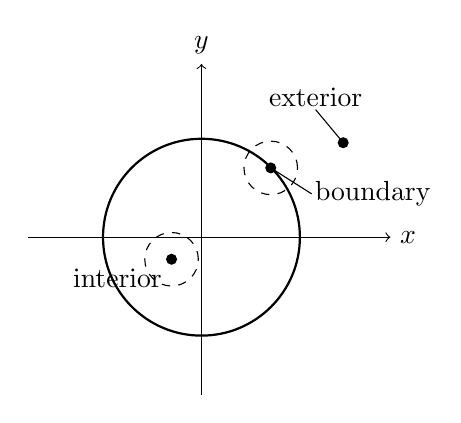
\begin{tikzpicture}[scale=1.0]
  \draw[->] (-2.2,0) -- (2.4,0) node[right] {$x$};
  \draw[->] (0,-2.0) -- (0,2.2) node[above] {$y$};
  \draw[thick] (0,0) circle (1.25);
  \coordinate (pint) at (-0.38,-0.28);
  \coordinate (pbd) at (0.88,0.88);
  \fill (pint) circle (2pt) node[below left] {interior};
  \fill (pbd) circle (2pt);
  \fill (1.8,1.2) circle (2pt);
  \draw[dashed] (pint) circle (0.34);
  \draw[dashed] (pbd) circle (0.34);
  \draw[thin] (pbd) -- (1.40,0.55);
  \node[anchor=west,fill=white,inner sep=1pt] at (1.40,0.55) {boundary};
  \draw[thin] (1.8,1.2) -- (1.45,1.62);
  \node[anchor=south,fill=white,inner sep=1pt] at (1.45,1.62) {exterior};
\end{tikzpicture}
\caption{Interior points have a small ball inside the set; boundary points never do.}
\end{figure}

\section{Open and closed sets}

\begin{definition}
A set \(E\subseteq\mathbb R^n\) is \vocab{open} if every point of \(E\) is an interior point.  It is \vocab{closed} if its complement is open.
\end{definition}

The two words are not opposites in the everyday sense.  A set can be both open and closed, or neither open nor closed.

\begin{example}
In \(\mathbb R\), the interval \((0,1)\) is open but not closed, \([0,1]\) is closed but not open, \([0,1)\) is neither open nor closed, and both \(\varnothing\) and \(\mathbb R\) are both open and closed.
\end{example}

\begin{proposition}
A set \(E\subseteq\mathbb R^n\) is closed if and only if it contains all its boundary points.
\end{proposition}

\begin{proof}[Proof skeleton]
If \(E\) is closed, its complement is open, so no boundary point can lie in the complement; hence every boundary point lies in \(E\).  Conversely, if \(E\) contains all boundary points, then any point outside \(E\) is not an interior point of \(E\) and not a boundary point, so it is exterior.  Thus the complement is open.
\end{proof}

\section{Accumulation points and closure}

\begin{definition}
A point \(P\) is an \vocab{accumulation point} of \(E\) if every punctured ball
\[
  B_\delta(P)\setminus\{P\}
\]
contains a point of \(E\).  The \vocab{closure} of \(E\), denoted \(\overline E\), is the union of \(E\) with all its accumulation points.
\end{definition}

\begin{proposition}[Sequential test]
For \(E\subseteq\mathbb R^n\), a point \(P\) lies in \(\overline E\) if and only if there is a sequence \((P_k)\) in \(E\) such that \(P_k\to P\).
\end{proposition}

\begin{proof}[Proof skeleton]
If \(P\in\overline E\), choose \(P_k\in E\cap B_{1/k}(P)\), using \(P_k=P\) if \(P\in E\) and necessary.  Then \(P_k\to P\).  Conversely, if \(P_k\in E\) and \(P_k\to P\), then every ball around \(P\) contains some \(P_k\), so \(P\) is in the closure.
\end{proof}

This gives the most useful closed-set criterion:
\[
  E\text{ is closed}\quad\Longleftrightarrow\quad
  \text{every convergent sequence in }E\text{ has its limit in }E.
\]

\section{Boundedness and compactness}

\begin{definition}
A set \(E\subseteq\mathbb R^n\) is \vocab{bounded} if it is contained in some ball \(B_R(0)\).  It is \vocab{compact} if every open cover of \(E\) has a finite subcover.
\end{definition}

In \(\mathbb R^n\), compactness has a simpler working form.

\begin{theorem}[Heine--Borel]
A subset \(K\subseteq\mathbb R^n\) is compact if and only if it is closed and bounded.
\end{theorem}

For computation, compactness is an existence machine.  It makes "largest," "smallest," and "convergent subsequence" statements true.

\begin{theorem}[Extreme value theorem]
If \(K\subseteq\mathbb R^n\) is compact and \(f:K\to\mathbb R\) is continuous, then \(f\) attains a maximum and a minimum on \(K\).
\end{theorem}

\begin{example}
The function \(f(x,y)=x^2+y^2\) has a maximum and a minimum on the closed disk \(x^2+y^2\le1\).  It has a minimum but no maximum on the open disk \(x^2+y^2<1\).  The missing boundary is exactly where the supremum would be reached.
\end{example}

\section{Connectedness and path-connectedness}

\begin{definition}
A set \(E\) is \vocab{connected} if it cannot be written as the union of two nonempty separated pieces.  It is \vocab{path-connected} if for any two points \(P,Q\in E\), there is a continuous curve \(\gamma:[0,1]\to E\) with \(\gamma(0)=P\) and \(\gamma(1)=Q\).
\end{definition}

Path-connectedness implies connectedness.  In the elementary domains of multivariable calculus, the two often coincide, but they are not the same in general.

A \vocab{region} in many calculus texts usually means an open connected subset of \(\mathbb R^n\), sometimes together with a piecewise smooth boundary when integration is involved.

\section{What this vocabulary controls}

The words in this note are not decorative definitions.  They decide which theorems are legal:
\[
\begin{array}{c|c}
\text{open set} & \text{local perturbations stay inside the domain}\\
\text{closed set} & \text{limits of internal sequences remain inside}\\
\text{compact set} & \text{continuous functions attain extrema}\\
\text{boundary} & \text{where constraints and integration surfaces live}\\
\text{connectedness} & \text{where one can move without jumping}
\end{array}
\]
When later notes discuss limits, tangent planes, extrema, or multiple integrals, these are the hidden hypotheses that make the calculations legitimate.
